\section{Zielsetzung}
In diesem Veruch wird die Erzeugung freier Elektronen durch Erhitzen eines
Metalles untersucht, dieses Phänomen wird auch als glühelektrischer Effekt
bezeichnet. Von besonderem Interesse ist dabei die Temperaturabhängigkeit, sowie
die Austrittsarbeit, die Materialabhängig ist. Diese Austrittsarbeit soll
in diesem Versuch für das Metall Wolfram bestimmt werden.
Da freie Elektronen sehr schnell mit den Luftmolekülen wechselwirken, wird dieser
Versuch im Hochvakuum durchgeführt. Um diese Bedingung zu realisieren wird eine
Hochvakuumdiode verwendet.

\section{Theorie}
Metalle haben eine hohe elektrische Leitfähigkeit, dies kann dadurch erklärt werden, dass
das Metallinnnere durch einen Potentialtopf wie in Abbildung \ref{fig:topf} beschrieben werden kann,
in dem sich die Elektronen kräftefrei bewegen können. Damit ein Elektron
diesen Potentialtopf verlassen kann benötigt es die sogenannte Austrittsarbeit
$e_{0}\xi$ ($e_{0}$= Elementarladung) um gegen das Potential $\xi$ anzulaufen.
\begin{figure}
  \centering
  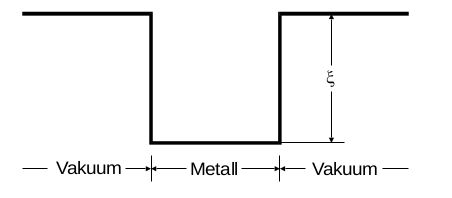
\includegraphics[height=3cm]{potentialtopf.png}
  \caption{Potentialtopfmodell eines Metalles}
  \label{fig:topf}
  \cite{skript}.
\end{figure}

Hier stellt sich die Frage, ob die Elektronen auch spontan genügend Energie besitzen
können um den Potentialtopf zu verlassen. Dazu sind zunächst zwei Aussagen wichtig:\\
1) Elektronen können nur diskrete Energiewerte annehmen.\\
2) Das Pauli-Prinzip besagt, dass jeder mögliche Zustand mit der Energie $E$ höchstens
\:\:\: von zwei Elektronen mit entgegengesetztem Spin eingenommen werden kann.\\

Die Fermi-Dirac-Verteilung gibt an, mit welcher Wahrscheinlichkeit ein Zustand der
Energie $E$ bei einer Temperatur $T$ besetzt wird. Sie wird durch die Funktion
\begin{equation}
  f(E)=\frac{1}{\exp\Bigl(\frac{E-\xi}{kT}\Bigr)+1}
  \label{eqn:fermi1}
\end{equation}
beschrieben. An dieser Formel kann man erkennen, dass das Elektron mindestens die Energie
$\xi+e_{0}\phi$ benötigt, um die Metalloberfläche zu verlassen. Dabei gibt $\phi$
die Potentialdifferenz zwischen Außenraum- und Innenraum des Potentialtopfes an.
Experimente haben ergeben, dass dieser Wert sehr groß ist, weshalb die
Exponentialfunktion im Nenner sehr stark wächst.
Für enrgiereiche Elektronen die das Metall verlssen können kann die Näherung
\begin{equation}
  f(E)=\exp\Bigl(\frac{\xi-E}{kT}\Bigr)
  \label{eqn:fermi2}
\end{equation}
verwendet werden.

\begin{figure}[H]
  \centering
  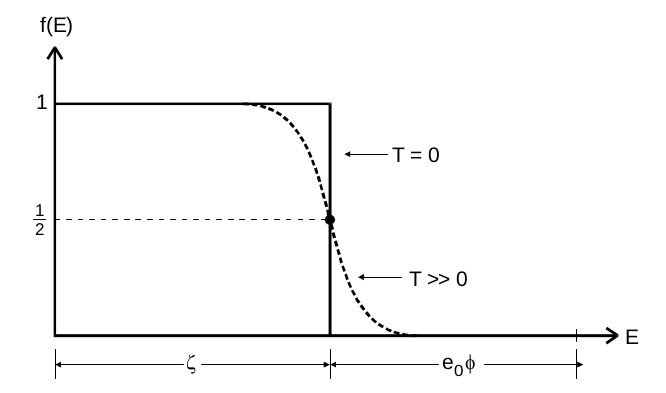
\includegraphics[height=5cm]{Fermi.png}
  \caption{Fermi-Diracksche Verteilungsfunktion.\\
  Gestrichelte Linie für T>>0 und durchgezogene Linie für T=0 (absoluter Nullpunkt)}
  \label{fig:fermi}
  \cite{skript}.
\end{figure}

Wie schon erwähnt wird für diesen Versuch eine Hochvakuumdiode verwendet. Hier ist
in ein vakuumiertes Glasgefäß eine Anode und Kathode eingelassen. Um den Elektronen
nun genügend Energie zuzuführen um das Metall zu verlassen wird die Kathode mit Hilfe einer
Heizspannung auf 1000-3000\;K erhitzt. Die austretenden Elektronen werden dann "abgesaugt", dies geschieht
über die positiv geladene Anode. Der Strom an der Anode ist nun ein Maß für die
ausgetretenen Elektronen.

\begin{figure}[H]
  \centering
  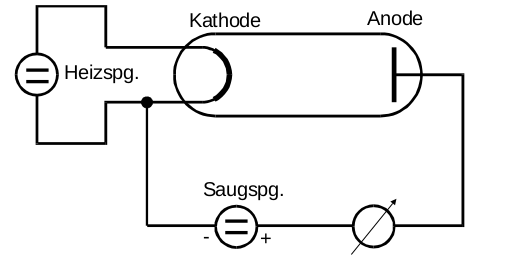
\includegraphics[height=5cm]{Aufbau.png}
  \caption{Aufbau einer Hochvakuumdiode}
  \label{fig:vakuum}
  \cite{skript}.
\end{figure}

Wird nun die Heizspannung gegen den gemessenen Strom zwischen Anode und Kathode aufgetragen
ergibt sich eine Kennlinie.

\begin{figure}[H]
  \centering
  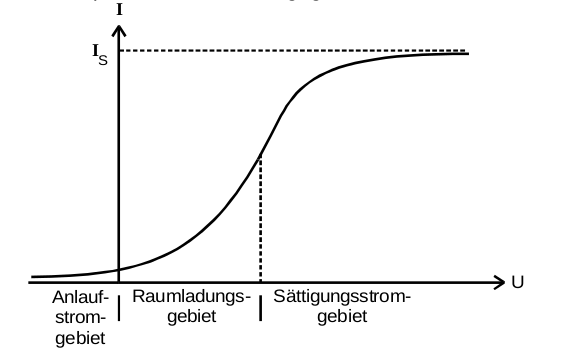
\includegraphics[height=6cm]{Kennlinie.png}
  \caption{Kennlinie einer Hochvakuumdiode}
  \label{fig:kenn}
  \cite{skript}.
\end{figure}

Diese Kennlienie lässt sich in drei Gebiete unterteilen: Anlaufgebiet, Raumladungsgebiet und
Sättigungsgebiet.\\
\\
\textbf{Anlaufgebiet:}\\
Es ist zu erkennen, dass selbst für kleine Gegenspannungen ein Stromfluss existiert.
Dieser lässt sich darüber begründen, dass die austretenden Elektronen eine statistisch
verteilte Energie besitzen. Es gibt also Elektronen, die genügend Enegie beitzen
um ein kleines Gegenfeld zu überwinden. Die Stromdichte für dieses Gebiet lässt sich
ausdrücken als
\begin{equation}
  j(V)=const\exp\Bigl({\frac{-e_{0}V}{k_{B}T}}\Bigr)
  \label{eqn:anlauf}
\end{equation}
und ist von der Gegenpannung $V$ und der Temperatur $T$ abhängig.
\\

\textbf{Raumladungsgebiet:}\\
In diesem Bereich erreichen nicht alle Elektronen die Anode und das Ohmsche Gesetz
($U=R\cdot I$) ist nicht gültig. Denn aufgrund der Kontinuitätsgleichung
\begin{equation}
  j=  -\rho v
\end{equation}
muss $\rho$ überall konstant sein. Da die Elektronen aber zur Anode hin beschleunigt werden
ist ihre Geschwindigkeit in Nähe der Anode größer. Also nimmt dort die Raumladungsdichte
$\rho$ ab. Anschaulich gesprochen erreichen die Feldlinien der Anode die Kathode nicht mehr,
sondern enden an den Raumladungselektronen. Somit werden die emittierten Elektronen
nicht mehr von dem Anodenfeld erfasst.
In diesem Bereich gilt also anstelle des Ohnschen Gesetzes das
Langmuir-Schottkysche Raumladungsgesetz:
\begin{equation}
  j=\frac{4}{9}\epsilon_{0}\sqrt{2e_{0}/m_{0}}*\frac{V^{(3/2)}}{a²}.
  \label{eqn:lang}
\end{equation}
$j \sim V^{(3/2)}$ ist eine Näherung, die sich durch die Herleitung ergibt.
 Weitere Zusammenhänge in einer Hochvakuumdiode sind im Folgenden dargestellt.
 \begin{figure}[H]
   \centering
   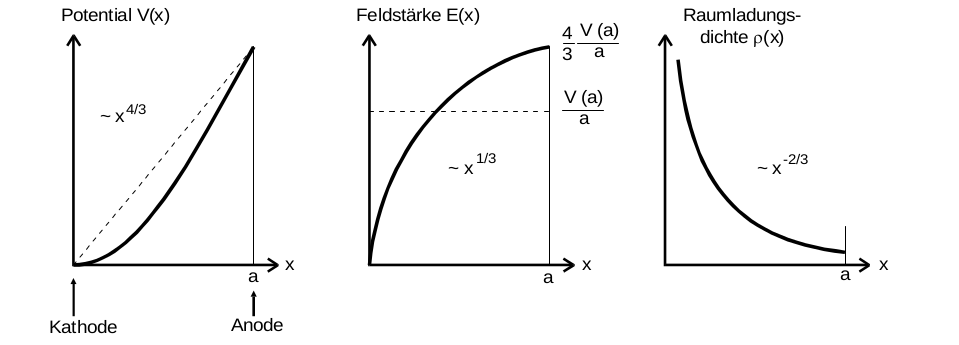
\includegraphics[height=5cm]{diagramm.png}
   \caption{Ortsabhängigkeit des Potentials V, der Fledstärke E und der Raumladungsdichte $\rho$
   im Raumladungsgebiet einer Hochvakuumdiode}
   \label{fig:diagramm}
   \cite{skript}.
 \end{figure}

\textbf{Sättigungsgebiet:}\\
Jetzt erreichen alle Elektronen die Anode. Der Grenzstrom ist nun nur von der
Austrittsarbeit und der Temperatur abhängig. In diesem Bereich gilt die
Richardson-Gleichung:
\begin{equation}
  j_{s}(T)= 4 \pi \frac{e_{0}m_{0}k²}{h³}T²\exp{\Bigl(\frac{-e_{0}\phi}{kT}\Bigr)}
  \label{eqn:satt}
\end{equation}
\\
\\


Aus der Leistungsbilanz des Heizstromfadens und dem Enrgiesatz ergibt sich folgende Formel
für die Kathodentemperatur:
\begin{equation}
  I_{f}U_{f}=f \eta \sigma\; T^{4}+N_{WL}.
  \label{temperatur}
\end{equation}
Dabei ist $f$ die emittierende Kathodenoberfläche, $\eta$ der Emissionsgrad der Oberfläche,
$\sigma$ die Stefan-Boltzmannsche Strahlungskonstante und $N_{WL}$ wurde auf $\SI{1}{\W}$
abgeschätzt.
\label{sec:Theorie}
